\documentclass[tikz,border=4pt]{standalone}
\usepackage{amsmath}
\begin{document}
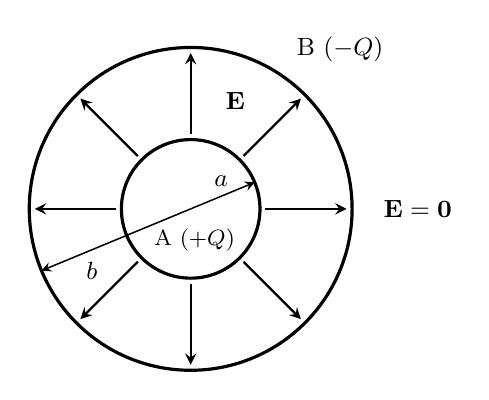
\begin{tikzpicture}[>=stealth, thick, scale=1.0]
  % Inner cylinder A (radius a = 0.88) and outer cylinder B (radius b = 2.05)
  \draw[line width=1.15pt] (0, 0) circle (0.88);
  \draw[line width=1.15pt] (0, 0) circle (2.05);

  % Radial electric field arrows between a and b (8 directions)
  \foreach \ang in {0, 45, 90, 135, 180, 225, 270, 315} {
    \draw[->, line width=0.8pt] ({\ang}:0.95) -- ({\ang}:1.98);
  }

  % Radius labels along clear angles
  \draw[->, line width=0.55pt] (0, 0) -- (22.5:0.88);
  \node[font=\small] at (42:0.52) {$a$};
  \draw[->, line width=0.55pt] (0, 0) -- (-157.5:2.05);
  \node[font=\small] at (-148:1.48) {$b$};

  % Labels A, B, +Q, -Q, E, E=0
  \node[font=\footnotesize] at (0.05, -0.40) {$\mathrm{A}\ (+Q)$};
  \node[above right, font=\small] at (55:2.12) {$\mathrm{B}\ (-Q)$};
  \node[font=\small] at (67.5:1.48) {$\mathbf{E}$};
  \node[right, font=\small] at (2.32, 0) {$\mathbf{E} = \mathbf{0}$};
\end{tikzpicture}
\end{document}
